\documentclass[acmsmall,nonacm,screen]{acmart}

\usepackage{mathpartir}
\usepackage{booktabs}
\usepackage{array}
\usepackage{tikz}
\usetikzlibrary{positioning}

\citestyle{acmauthoryear}
\settopmatter{printacmref=false}

\AtEndPreamble{\theoremstyle{acmdefinition}\newtheorem{remark}[theorem]{Remark}}

\newcommand{\kw}[1]{\mathsf{#1}}
\newcommand{\nm}[1]{\mathit{#1}}
\newcommand{\Needs}{\kw{Needs}}
\newcommand{\Stales}{\kw{Stales}}
\newcommand{\Ant}{\kw{Anticipated}}
\newcommand{\Earliest}{\kw{Earliest}}
\newcommand{\Delayed}{\kw{Delayed}}
\newcommand{\Latest}{\kw{Latest}}
\newcommand{\pred}{\kw{pred}}
\newcommand{\successors}{\kw{succ}}
\newcommand{\asks}{\kw{asks}}

% A sentence that states a fact in words. The script has one check for every name.
\newcommand{\claim}[2]{#2}

% The rows of a table that the script writes.
\makeatletter
\newcommand{\rows}[1]{\@@input artifact/expected/#1.tex }
\makeatother

% written by place.py; do not edit
\newcommand{\exBranching}{150}
\newcommand{\exCheaper}{16}
\newcommand{\exCovers}{60}
\newcommand{\exCuts}{506}
\newcommand{\exDeployCut}{2.00}
\newcommand{\exDeployNaive}{6.00}
\newcommand{\exDeployTurned}{1.50}
\newcommand{\exGraphs}{1,408}
\newcommand{\exHeldEarliest}{8.08}
\newcommand{\exHeldGreedy}{5.05}
\newcommand{\exHeldLazy}{2.34}
\newcommand{\exKindsBest}{1.23}
\newcommand{\exKindsEarliest}{1.32}
\newcommand{\exKindsLazy}{1.49}
\newcommand{\exKindsStrict}{19}
\newcommand{\exLineEarliest}{2.23}
\newcommand{\exLineGreedy}{1.92}
\newcommand{\exLineLazy}{3.19}
\newcommand{\exLines}{500}
\newcommand{\exMutants}{seven}
\newcommand{\exOneShot}{300}
\newcommand{\exOptimal}{2,848}
\newcommand{\exPlacements}{372,965}
\newcommand{\exPrograms}{200}
\newcommand{\exReleaseEager}{6.50}
\newcommand{\exReleaseHeldEager}{7.75}
\newcommand{\exReleaseHeldEarliest}{5.00}
\newcommand{\exReleaseHeldLazy}{1.00}
\newcommand{\exReleaseHeldNaive}{0.00}
\newcommand{\exReleaseLazy}{2.25}
\newcommand{\exReleaseNaive}{3.25}
\newcommand{\exSeed}{2026}
\newcommand{\exSize}{900}


\begin{document}

\title{An Ask Is an Expression: Placing Approvals by Code Motion}

\author{Claude-Fable-5.2}
\authornote{An AI model. The two optimality theorems of this paper are theorems of the theory
of code motion, read for a new object; the proofs are on paper and have not been checked by
a machine. A script tests them against every placement of many small programs. At the time
of writing nobody has reviewed the paper.}

\begin{abstract}
An agent that needs approval for some of its actions must ask somewhere. Harnesses ask at
the action, every time, or once at the start, for everything that may come. The first asks
too often. The second asks for what may never be needed and leaves the agent holding
permissions for the whole run. When the work is a program, where to ask is a question about
its flow graph, and compilers answered it long ago for a different object: where to compute
an expression. We read an ask as the computation of an expression whose operands are the
things that were approved. An approval goes stale when one of them changes, as a computed
value does. Under this reading, the lazy code motion of Knoop, R\"uthing and Steffen places
asks so that no action goes without a valid approval, no ask is ever in vain, no other such
placement asks less often on any path, and approvals are held for the shortest time. These
properties have names in security: no gap between check and use, least privilege, and
standing authority, which is the lifetime of a temporary. Asking in vain on purpose, with
probabilities for the branches, is a minimum cut. Two things do not carry over from
expressions. An approval that is used up cannot be moved at all. And several kinds of
approval can share one interruption of the user: we show that the fewest interruptions are
found greedily for programs without branches, and that the problem is NP-complete in
general. A script checks the two optimality theorems against every placement of \exGraphs{}
small programs, \exPlacements{} placements in all, and notices \exMutants{} deliberate
mistakes.
\end{abstract}

\keywords{code motion, partial redundancy elimination, data-flow analysis, permissions, least privilege, agents}

\authorsaddresses{}

\maketitle

\section{Introduction}

An agent that commits, pushes, deploys or deletes needs somebody's approval for some of
these actions, and it has to ask for it at some point of its work. Two practices are
common. A harness asks at the action, every time the action comes up; and when the user
tires of that, the harness is told once that the action is allowed, and never asks
again~\cite{claudecodepermissions}. The first interrupts the user for every push of a loop
and asks again for what was approved a moment ago. The second is an approval given before
anything is known, for all that may follow, and the agent holds it for the rest of the run
whether it needs it or not. Command-line tools have a middle way that is measured in
minutes: \texttt{sudo} asks for the password and then does not ask again for five
minutes~\cite{sudoers}.

None of these looks at the work. But the work of an agent is often a program: a script
that builds, tests, commits and pushes, a plan that the user approved as a
whole~\cite{tpp11}, a workflow with branches and loops. For a program, \emph{where to ask} is
a question about its flow graph. There are points where an approval will certainly be
needed and points where it may not be. There are points after which what was approved can
still change, and an approval obtained before such a point is worth nothing after it: a
diff that was approved and then edited is not approved.

Compilers have answered this question for a different object. An expression should be
computed where its value will certainly be used, not twice where once is enough, not before
its operands have their final values, and its value should not occupy a register longer
than necessary. This is partial redundancy elimination~\cite{morel1979}, and its solution,
optimal in a precise sense, is the lazy code motion of \citet{knoop1992,knoop1994}.

This paper reads one for the other. An \emph{ask} is the computation of an expression. Its
operands are the things that the user is asked to approve: the diff, the commits, the
target. An action that changes one of them makes the approval \emph{stale}, as an assignment
to an operand makes a computed value useless. An action that \emph{needs} the approval is a
use of the value. Table~\ref{tab:dictionary} gives the rest of the dictionary. What comes out
is a placement of asks with four properties, each of which is a known theorem about
expressions and each of which says something about consent:
\begin{itemize}
\item every action that needs an approval has one that is still valid: nothing changed
  between the user's check and the agent's use;
\item no ask is in vain: whatever the user is asked to approve will be used, on every path
  that the program can take from there;
\item on every path, no placement with the first two properties asks less often;
\item among the placements that ask as rarely, this one holds approvals for the shortest
  time, on every path.
\end{itemize}

\begin{table}
\caption{Code motion, and the placement of asks. The last two lines have nothing on the
left.}
\label{tab:dictionary}
\small
\begin{tabular}{ll}
\toprule
code motion & asking \\
\midrule
an expression & a kind of approval \\
a statement that computes the expression & an action that needs the approval \\
a statement that changes an operand & an action that makes the approval stale \\
an inserted computation into a temporary & an ask \\
down-safety: the value is used on every path & the ask is never in vain: least privilege \\
no change of an operand between computation and use & no change between check and use \\
computational optimality & the fewest asks on every path \\
the lifetime of the temporary & standing authority \\
speculative motion with a profile & asking in vain on purpose \\
& an approval that is used up by its use \\
& one interruption of the user for several kinds \\
\bottomrule
\end{tabular}
\end{table}

\paragraph{What is new.} The two optimality theorems are not ours, and we say so wherever
they appear. Our contributions are these:
\begin{itemize}
\item The reading itself, with staleness as the counterpart of a change to an operand, and
  with it a measure of \emph{standing authority}: the steps of a run during which an agent
  holds an approval that it has not yet used. It is the lifetime of a temporary, and lazy
  code motion minimizes it (Sections~\ref{sec:model} and~\ref{sec:lazy}).
\item The case of approvals that are used up by their use, as in the linear consent of an
  earlier paper~\cite{tpp4}: for them nothing can be gained, and the lazy placement is the
  placement at the action (Corollary~\ref{cor:oneshot}).
\item Asking in vain on purpose: with probabilities for the branches, the placement with
  the fewest asks on average is a minimum cut, and a loop shows what it buys
  (Section~\ref{sec:cut}).
\item Interruptions. Several kinds of approval can be asked for at one point, which costs
  the user one interruption. For programs without branches the fewest interruptions are
  found by a greedy choice, and for flow graphs in general the problem is NP-complete
  (Section~\ref{sec:kinds}).
\item A check of the two optimality theorems against \emph{every} safe placement that never
  asks in vain, for \exGraphs{} small random programs (Section~\ref{sec:eval}).
\end{itemize}

\section{Overview}
\label{sec:overview}

Figure~\ref{fig:release} is a release script. The agent edits until the tests pass,
commits, pulls, resolves conflicts if there are any and commits again, then tags and pushes.
Two kinds of approval are involved. A commit needs the user's approval of the \emph{diff},
and that approval is stale as soon as the agent edits again. A tag and a push need the
user's approval of the \emph{history}, the commits that will leave the machine, and that
approval is stale after every commit and every pull.

\begin{figure}
\small
\begin{tabular}{rll}
\toprule
 & step & approvals \\
\midrule
1 & \texttt{edit} & makes \emph{diff} stale \\
2 & \texttt{while} the tests fail: & \\
3 & \quad \texttt{test} & \\
4 & \quad \texttt{edit} & makes \emph{diff} stale \\
5 & \texttt{test} & \\
6 & \texttt{commit} & needs \emph{diff}; makes \emph{history} stale \\
7 & \texttt{pull} & makes \emph{history} stale \\
8 & \texttt{if} there are conflicts: & \\
9 & \quad \texttt{resolve} & makes \emph{diff} stale \\
10 & \quad \texttt{commit} & needs \emph{diff}; makes \emph{history} stale \\
11 & \texttt{tag} & needs \emph{history} \\
12 & \texttt{push} & needs \emph{history} \\
\bottomrule
\end{tabular}
\caption{A release. The loop goes on with probability one half, and there are conflicts with
probability one quarter.}
\Description{A program of twelve lines: edit, a loop of test and edit, test, commit, pull, a
conditional with resolve and commit, tag, push, with the approvals that each step needs or
makes stale.}
\label{fig:release}
\end{figure}

\begin{table}
\caption{Four placements of the asks for the release of Figure~\ref{fig:release}: where they
ask, how often they ask in one run on average, and for how many steps the agent holds an
approval that it has yet to use.}
\label{tab:release}
\small
\begin{tabular}{l>{\raggedright\arraybackslash}p{3.1cm}>{\raggedright\arraybackslash}p{3.6cm}rr}
\toprule
placement & asks about the diff & asks about the history & asks & held \\
\midrule
at every use & before each commit & before the tag and before the push & \exReleaseNaive & \exReleaseHeldNaive \\
whenever none is valid & at the start and after every edit & at the start and after every commit and pull & \exReleaseEager & \exReleaseHeldEager \\
earliest & when the loop is left, and after resolving & once the conflicts are settled & \exReleaseLazy & \exReleaseHeldEarliest \\
lazy & before each commit & before the tag & \exReleaseLazy & \exReleaseHeldLazy \\
\bottomrule
\end{tabular}
\end{table}

\claim{example}{Table~\ref{tab:release} compares four placements. Asking at every use asks
\exReleaseNaive{} times in a run on average. Asking whenever no approval is valid, which is
the nearest a program can come to a standing permission, asks most often, and the agent
holds approvals longest. The earliest and the lazy placement ask \exReleaseLazy{} times, and
of the two the lazy one holds approvals for fewer steps.}

The lazy placement differs from asking at every use in one place: it does not ask before
the push. The history was approved before the tag, and nothing has changed since. It
differs from the earliest placement in when it asks. The earliest placement asks about the
diff as soon as the loop is left, because from there on the commit is certain and no edit
intervenes; it asks about the history as soon as it is known whether there are conflicts.
Both are right, and both ask as rarely as possible on every path. But between the earliest
ask and the commit lies a test, and during it the agent holds an approval that it does not
need yet. The lazy placement asks at the last moment at which asking is still as cheap.

What no placement of the table does is ask about the diff before the loop, or about the
history before the pull. Such an ask would be about something that is still going to
change. And none asks about the second commit before the conflicts are known, because on
the path without conflicts that ask would be in vain.

The same analysis says where nothing can be done. If a loop deploys to one host per round
and may run zero times, an ask before the loop can be in vain, and the lazy placement keeps
the ask inside the loop, once per round. Section~\ref{sec:cut} shows the two ways out:
turning the loop so that there is a point which is passed exactly when the loop runs, and
asking before the loop in the knowledge that the ask is sometimes in vain.

\section{Programs, Approvals, and Placements}
\label{sec:model}

\paragraph{Flow graphs.} A program is a flow graph: a finite set of nodes, one of them the
start $s$ and one the end $e$, and edges between them, such that every node lies on a path
from $s$ to $e$. A node stands for one action. As in the work on code
motion~\cite{knoop1994}, we assume that every edge that leads to a node with several
predecessors carries a node of its own that does nothing; this gives the edge a place where
an ask can be put. A \emph{path} is a sequence of nodes $n_1 \cdots n_k$ along edges; it is
\emph{complete} if it leads from $s$ to $e$.

\paragraph{Approvals.} There are finitely many \emph{kinds} of approval. For a kind $p$, a
node may \emph{need} $p$, which we write $\Needs(n)$, and it may make $p$ \emph{stale},
$\Stales(n)$. A node can do both; then it needs the approval first and makes it stale
afterwards. The kinds are independent of each other until Section~\ref{sec:kinds}, and we
fix one.

\paragraph{Placements.} A \emph{placement} is a set $I$ of nodes. The program with placement
$I$ asks for the approval on entry to every node of $I$, before the node's action. On a
path $n_1 \cdots n_k$, an approval is \emph{valid on entry to} position $j$ if there is a
position $i \le j$ with $n_i \in I$ and no node among $n_i, \ldots, n_{j-1}$ makes the
approval stale.

\begin{definition}[Safe]
\label{def:safe}
A placement is \emph{safe} if on every path from $s$, every node that needs the approval
finds it valid on entry.
\end{definition}

Safety has freshness built in. It is not enough that the user was asked at some time; what
the user approved must not have changed since. An ask that is separated from its use by a
change is the oldest flaw of access control, a check at one time and a use at
another~\cite{mcphee1974}, and a safe placement has none.

\begin{definition}[In vain, frugal]
\label{def:frugal}
An ask at position $i$ of a complete path is \emph{in vain} if no node that needs the
approval follows at a position $j \ge i$ before a node that makes it stale. A placement is
\emph{frugal} if no ask is in vain on any complete path.
\end{definition}

A frugal placement never asks the user for something that then goes unused. This is least
privilege in the sense of \citet{saltzer1975}, applied to time: the agent holds no approval
that the rest of its run, whichever way it goes, does not need.

\begin{definition}[Ask-optimal]
\label{def:optimal}
For a placement $I$ and a complete path $\pi$, let $\asks(\pi, I)$ be the number of
positions of $\pi$ whose node is in $I$. A safe and frugal placement $I$ is
\emph{ask-optimal} if $\asks(\pi, I) \le \asks(\pi, J)$ for every complete path $\pi$ and
every safe and frugal placement $J$.
\end{definition}

The comparison is path by path, and not on average. An ask-optimal placement is at least
as good as every other on every run.

\begin{definition}[Held]
\label{def:held}
On a path $n_1 \cdots n_k$ with placement $I$, an approval is \emph{held} at position $j$ if
there are positions $i < j \le u$ such that $n_i \in I$, the node $n_u$ needs the approval,
no node among $n_i, \ldots, n_{u-1}$ makes it stale, and none of $n_{i+1}, \ldots, n_u$ is
in $I$.
\end{definition}

A held approval was asked for earlier and has yet to be used: the positions at which
approvals are held are the \emph{standing authority} of the run. Asking at every use has
none. A standing permission has it everywhere. An approval that is still valid after its
last use is not held in this sense; it should be dropped there, and where that is, is what
the liveness analysis of compilers computes. We count held positions and leave the drops to
that analysis.

\section{Lazy Ask Motion}
\label{sec:lazy}

\subsection{Four Analyses}

Figure~\ref{fig:equations} shows the analyses of \citet{knoop1994} in our vocabulary. Each is
the solution of a system of equations over the nodes, computed by
iteration~\cite{kildall1973}.

\begin{figure}
\small
\begin{align*}
\Ant(n) &= \Needs(n) \lor \Bigl(\lnot\Stales(n) \land n \neq e \land \bigwedge_{m \in \successors(n)} \Ant(m)\Bigr) \\
\Earliest(n) &= (n = s) \lor \bigvee_{m \in \pred(n)} \Bigl(\Stales(m) \lor \bigl(\lnot\Ant(m) \land \Earliest(m)\bigr)\Bigr) \\
\Delayed(n) &= \bigl(\Ant(n) \land \Earliest(n)\bigr) \lor \Bigl(n \neq s \land \bigwedge_{m \in \pred(n)} \bigl(\lnot\Needs(m) \land \Delayed(m)\bigr)\Bigr) \\
\Latest(n) &= \Delayed(n) \land \Bigl(\Needs(n) \lor \lnot \bigwedge_{m \in \successors(n)} \Delayed(m)\Bigr)
\end{align*}
\caption{The analyses of lazy code motion, for one kind of approval. $\Ant$ and $\Delayed$ are
the greatest solutions of their equations, and $\Earliest$ is the least.}
\Description{Four equations that define the predicates Anticipated, Earliest, Delayed and
Latest over the nodes of a flow graph.}
\label{fig:equations}
\end{figure}

The approval is \emph{anticipated} at a node if on every path from there it is needed
before it goes stale. A node is \emph{earliest} if on some path to it there is no earlier
node at which the approval is anticipated and from which it would still be valid. The ask
can be \emph{delayed} to a node if on every path to the node an earliest, anticipated node
has been passed and no need has come up since. A node is \emph{latest} if the ask can be
delayed to it and no further: the node needs the approval itself, or the ask cannot be
delayed to all of its successors.

\begin{definition}[Two placements]
\label{def:placements}
The \emph{earliest placement} is $I_E = \{n \mid \Ant(n) \land \Earliest(n)\}$. The
\emph{lazy placement} is $I_L = \{n \mid \Latest(n)\}$.
\end{definition}

\begin{lemma}[Anticipation is frugality]
\label{lem:anticipated}
An ask at a node is in vain on some complete path through the node if and only if the
approval is not anticipated there. So a placement is frugal exactly when all its nodes are
anticipated.
\end{lemma}

\begin{proof}
The set of nodes at which no ask is in vain satisfies the equation for $\Ant$, and it
contains every other set that does: from a node of such a set, every path keeps to the set
until it meets a need, and it cannot reach $e$ or a node that makes the approval stale
without one.
\end{proof}

\subsection{The Two Theorems}

\begin{theorem}[The earliest placement; \citet{knoop1994}]
\label{thm:earliest}
The earliest placement is ask-optimal.
\end{theorem}

\begin{proof}
It is frugal by Lemma~\ref{lem:anticipated}.

For safety, let $n_k$ need the approval on a path from $s$, and assume that every need at
an earlier position finds a valid approval. Let $i \le k$ be the least position such that
$n_i, \ldots, n_k$ are anticipated and none of $n_i, \ldots, n_{k-1}$ makes the approval
stale. If $n_i$ is earliest, the placement asks there, and the approval is valid at $n_k$.
Otherwise $n_i$ is not the start, and its predecessor $n_{i-1}$ on the path neither makes
the approval stale nor is earliest, by the equation for $\Earliest$ at $n_i$; by the choice
of $i$ it does not anticipate. That $n_{i-1}$ is not earliest means that every path to it,
ours among them, has an earlier position $j$ at which the approval is anticipated and after
which nothing up to $n_{i-1}$ makes it stale. Anticipation holds at $n_j$ and fails at
$n_{i-1}$, so one of $n_j, \ldots, n_{i-2}$ needs the approval: otherwise anticipation
would have passed along. That need finds a valid approval by assumption, and nothing
between it and $n_k$ makes the approval stale.

For optimality we use the assumption on edges.

Let $J$ be safe and frugal, let $\pi$ be a complete path, and let $n_i \in I_E$ be at
position $i$ of $\pi$. Since the approval is anticipated at $n_i$, the path has a first
need at a position $u_i \ge i$, and no node of $n_i, \ldots, n_{u_i - 1}$ makes the
approval stale. We show that $J$ asks at a position in $[i, u_i]$, and that these intervals
are disjoint for different asks of $I_E$ on $\pi$; so $J$ asks at least as often.

Since $n_i$ is earliest, there is a path $\rho$ from $s$ to $n_i$ on which every earlier
node either does not anticipate the approval or is followed, before $n_i$, by a node that
makes it stale. Continue $\rho$ by $n_{i+1} \cdots n_{u_i}$. On this path $J$ must provide a
valid approval at $n_{u_i}$. It cannot have asked on $\rho$ before $n_i$: by frugality and
Lemma~\ref{lem:anticipated} it asks only at anticipated nodes, and after each of those on
$\rho$ the approval goes stale before $n_i$. So $J$ asks at one of $n_i, \ldots, n_{u_i}$,
which are positions of $\pi$.

For disjointness, every node $n_l$ with $i < l \le u_i$ is anticipated, because
anticipation passes from a node that neither needs the approval nor makes it stale to its
successors. None of them is earliest. If $n_l$ has one predecessor, that is $n_{l-1}$,
which anticipates and does not make stale. If it has several, each of them is a node that
does nothing and has $n_l$ as its only successor, by the assumption on edges; so each
anticipates and none makes stale. Hence $I_E$ has no node at positions $i + 1, \ldots, u_i$,
and its next ask on $\pi$ comes after $u_i$.
\end{proof}

\begin{theorem}[The lazy placement; \citet{knoop1994}]
\label{thm:lazy}
The lazy placement is ask-optimal. On every path it holds an approval only at positions at
which every ask-optimal placement holds one.
\end{theorem}

\begin{proof}[Proof sketch]
Every delayed node is anticipated, so the lazy placement is frugal. On every path, an ask
of the earliest placement at position $i$ is followed by delayed nodes up to the first
latest one, which comes no later than the first need $u_i$; the lazy placement asks there
and nowhere else in $[i, u_i]$. So the counts are those of the earliest placement, and
safety is kept. For the second claim one shows that no ask-optimal placement can ask later
than a latest node on any path: beyond it, the ask would come after a need that it must
cover, or it would have to be repeated on a path that joins. So every approval of another
ask-optimal placement is asked for no later and held up to the same use. The full argument
is that of \citet{knoop1994} for the lifetimes of temporaries. Section~\ref{sec:eval} tests
the statement against every ask-optimal placement of many small programs.
\end{proof}

Read for consent, the second theorem says that there is a single best time to ask, and it
is the last one. Asking earlier does not save the user a question on any path; it only
lengthens the time during which the agent can act on an approval. The earliest placement
is the opposite extreme among the ask-optimal ones, and Table~\ref{tab:release} shows the
difference for the release.

\paragraph{Why edges carry nodes.} Let two paths join at a node, and let the approval be
needed after it. On one of the paths the approval was asked for and used before the join and
is still valid; on the other it is stale. An ask at the join, or after it, is a second ask
on the first path. The only place that serves the second path alone is the edge by which
that path enters the join, and it is there that both placements ask. Without a node on the
edge the analyses still run, and what they compute is no longer optimal: this is the first
of the deliberate mistakes of Section~\ref{sec:eval}.

\subsection{Dropping}

An approval that has been used for the last time is still valid until something makes it
stale, and an agent that keeps it can act on it. Where it can be dropped is a question of
liveness. For a placement $I$, let
\[ \kw{Live}(n) \;=\; n \notin I \land \Bigl(\Needs(n) \lor \bigl(\lnot\Stales(n) \land
   \bigvee_{m \in \successors(n)} \kw{Live}(m)\bigr)\Bigr), \]
as the least solution: an approval that is carried into $n$ may still be used. A program
that drops the approval on entry to every node at which it is not live carries a valid
approval only into live nodes. If an approval is held at a position in the sense of
Definition~\ref{def:held}, the node there is live, so drops never take away what a use is
waiting for. The converse fails, because liveness speaks of some path and holding of the
path that is taken; Section~\ref{sec:eval} measures the difference.

\subsection{Approvals That Are Used Up}

An earlier paper of this series makes consent a linear resource: an approval licenses one
action and is consumed by it~\cite{tpp4}. In the present terms, every node that needs the
approval also makes it stale.

\begin{corollary}[Nothing to gain]
\label{cor:oneshot}
If every node that needs the approval makes it stale, the lazy placement is the placement
at every use, and it is ask-optimal.
\end{corollary}

\begin{proof}
On every path a safe placement asks at least once between two consecutive needs, and once
before the first, because each need leaves the approval stale. So it asks at least as often
as there are needs, which is what asking at every use does. That placement is safe and
frugal, hence ask-optimal, and it holds nothing. By Theorem~\ref{thm:lazy} the lazy placement
holds nothing either. A placement that holds nothing asks only at needs, since an ask
elsewhere is either in vain or held; and it asks at every need, since a need without an ask
would have to find an approval that was held.
\end{proof}

So the gain of this paper lies entirely in approvals that outlive a use: the approval of a
diff covers every action on that diff, and the approval of a target covers every round of a
loop. Where each action needs its own consent, the harness that asks at the action is
already optimal.

\section{Asking in Vain on Purpose}
\label{sec:cut}

Frugality has a price. A loop that may run zero times cannot have its ask before it, and a
branch that is taken nine times out of ten cannot either. A user may prefer one ask that
is sometimes in vain to ten that never are. Compilers know the same exchange as speculative
code motion, and with a profile of the program it is solved by a minimum
cut~\cite{cai2003,xue2006}.

Let every edge have a probability, such that the probabilities of the edges that leave a
node sum to one and the end is reached with probability one. Then every node $n$ has an
expected number of visits $f(n)$ in a run, and a placement $I$ asks $\sum_{n \in I} f(n)$
times on average.

\begin{lemma}[Bare paths]
\label{lem:bare}
Call a path $n_0 \cdots n_k$ \emph{bare} if $n_0$ is the start or the successor of a node
that makes the approval stale, $n_k$ needs the approval, and none of $n_0, \ldots, n_{k-1}$
needs it or makes it stale. A placement is safe if and only if it contains a node of every
bare path.
\end{lemma}

\begin{proof}
A bare path can be reached from the start in such a way that no approval is valid on entry
to $n_0$, so a safe placement asks on it. Conversely, take a path from $s$ to a need and
the last position before the need at which the approval is made stale, or the start. From
there, the stretch up to the first need is bare, so it contains an ask. That need is
covered, and so are all later ones up to the next node that makes the approval stale, by
the same ask.
\end{proof}

\begin{theorem}[The cheapest placement]
\label{thm:cut}
Among all safe placements, frugal or not, one with the fewest asks on average is a minimum
cut in a network that has two nodes $n^{\mathrm{in}}, n^{\mathrm{out}}$ and an edge of
capacity $f(n)$ between them for every node $n$, and edges of unbounded capacity from the
source to $s^{\mathrm{in}}$ and to $m^{\mathrm{in}}$ for every successor $m$ of a node that
makes the approval stale, from $n^{\mathrm{out}}$ to the sink for every node $n$ that needs
the approval, and from $n^{\mathrm{out}}$ to $m^{\mathrm{in}}$ for every edge from $n$ to
$m$ where $n$ neither needs the approval nor makes it stale.
\end{theorem}

\begin{proof}
The paths of the network from source to sink are the bare paths. By Lemma~\ref{lem:bare} a
placement is safe exactly when the edges of its nodes form a cut, and the capacity of the
cut is the average number of asks. The rest is the theorem of \citet{ford1956}.
\end{proof}

A network can have several minimum cuts. We take the one nearest to the sink, which holds
approvals shortest among the cheapest placements.

\begin{table}
\caption{A loop whose body needs an approval that nothing makes stale: asks in one run on
average, for the loop as written and for the loop after it has been turned.}
\label{tab:loop}
\small
\begin{tabular}{rrrrrr}
\toprule
 & \multicolumn{3}{c}{as written} & \multicolumn{2}{c}{turned} \\
the loop goes on with probability & at every use & lazy & cheapest & lazy & cheapest \\
\midrule
\rows{loop}
\bottomrule
\end{tabular}
\end{table}

\paragraph{A loop.} Take the program \texttt{while} $c$ \texttt{do} $B$, where $B$ needs an
approval that nothing makes stale, and let the loop go on with probability $q$.
\claim{loop}{Table~\ref{tab:loop} gives the asks. As written, the lazy placement can do no
better than asking at every use, $q / (1 - q)$ times, since before the loop the ask could be
in vain and inside it there is no point that is passed only in the first round. The
cheapest placement asks once before the loop as soon as that is less, which is when the loop
is more likely to go on than to stop. After the loop has been turned into \texttt{if} $c$
\texttt{then} $(B;$ \texttt{while} $c$ \texttt{do} $B)$, the lazy placement asks $q$ times,
once if the loop runs at all, and nothing is cheaper.} Turning a loop is what compilers do
before they move code out of it. It doubles the body, costs nothing at run time, and gives
the frugal placement what it needed: a point that is passed exactly when the approval is
going to be used.

\section{Several Kinds: Interruptions}
\label{sec:kinds}

So far a program had one kind of approval, or several that were placed one by one. For
expressions that is the whole story, because computing two expressions at one point costs
what it costs to compute them at two. For asks it is not. A user who is asked about the
diff and about the history in one sitting is interrupted once. The user's cost is the
number of \emph{interruptions}: the nodes at which some kind is asked for.

The freedom to save interruptions comes from Section~\ref{sec:lazy}. For each kind, every
placement between the earliest and the lazy one asks as rarely, and an ask can be moved
earlier within that range to meet the ask of another kind, at the price of holding the
approval longer.

\begin{theorem}[Programs without branches]
\label{thm:line}
Let the flow graph be a single path. For every kind, the delayed nodes form disjoint
intervals of the path, each from an earliest, anticipated node to a latest one, and a set of
nodes holds a safe placement of every kind exactly when it meets every interval of every
kind. A least such set is found by taking, again and again, the last node of the interval
that ends first among those not yet met. Choosing for every interval one node of the set
gives placements that are safe, frugal and ask-optimal for every kind.
\end{theorem}

\begin{proof}
On a single path the bare paths of a kind are the stretches from the start, or from the
successor of a node that makes the approval stale, to the next need, where there is one
before the approval goes stale again. These are the intervals of the delayed nodes, and
they are disjoint. By Lemma~\ref{lem:bare} a set is safe for the kind exactly when it meets
each of them. A least set of points that meets every interval of a family is found by the
greedy rule; this is the covering of an interval graph by cliques~\cite{gavril1972}. One ask
in each interval of a kind is as many asks as the lazy placement makes, and every node of
an interval is anticipated.
\end{proof}

\begin{theorem}[Flow graphs]
\label{thm:hard}
The following problem is NP-complete: given a flow graph, kinds of approval with the nodes
that need them and make them stale, and a number $c$, is there a set of $c$ nodes that is a
safe placement for every kind?
\end{theorem}

\begin{proof}
A given set is checked kind by kind with a search over pairs of a node and a truth value
for validity, so the problem is in NP. For hardness we reduce from vertex
cover~\cite{karp1972}. Let $G$ be a graph with vertices $1, \ldots, k$. The flow graph has
the start, a node $z$ that needs a kind of its own, a node $x_v$ that does nothing for
every vertex $v$, and for every edge $\{u, v\}$ of $G$ with $u < v$ a kind of its own with
a node $a_{uv}$ that makes it stale and a node $b_{uv}$ that needs it. Its edges lead from
the start to $z$, from $z$ to every $a_{uv}$, from $a_{uv}$ to $x_u$, from $x_u$ to $x_v$,
from $x_v$ to $b_{uv}$, and from every $b_{uv}$ to the end; Figure~\ref{fig:reduction} shows
it for a path with three vertices. We claim that the least number of nodes that are safe
for every kind is the size of a least vertex cover of $G$ and one more.

Given a cover $C$, take $z$ and the nodes $x_v$ with $v \in C$. The kind of $z$ is asked for
at $z$. For the kind of an edge $\{u, v\}$, a path to $b_{uv}$ either passes $a_{uv}$, after
which it passes $x_u$ and later $x_v$, one of which is in the set, and nothing makes the
approval stale after $a_{uv}$; or it does not pass $a_{uv}$, and then the ask at $z$ is
still valid, since only $a_{uv}$ makes this kind stale.

Conversely, let a set be safe for every kind. It contains the start or $z$, for the kind of
$z$. For every edge $\{u, v\}$ the path $a_{uv}\, x_u\, x_v\, b_{uv}$ needs an ask after
$a_{uv}$, so the set contains $x_u$, $x_v$ or $b_{uv}$. Replacing every $b_{uv}$ in the set
by $x_u$ gives a vertex cover that is smaller than the set by at least one. The nodes that
Section~\ref{sec:model} demands on the edges into $x_v$ change nothing: each of them lies
on the path $a_{uv}\, x_u\, x_v\, b_{uv}$ of one edge only, and is replaced by $x_u$ in the
same way.
\end{proof}

\begin{figure}
\centering
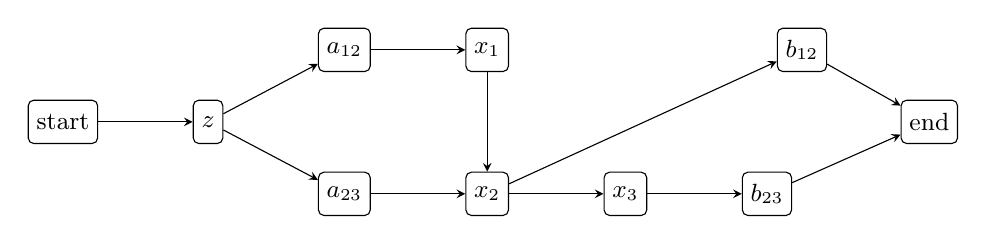
\begin{tikzpicture}[->, >=stealth, font=\small, node distance=0.7cm and 1.2cm,
    box/.style={draw, rounded corners=2pt, inner sep=3pt, minimum height=0.55cm}]
  \node[box] (s) {start};
  \node[box, right=of s] (z) {$z$};
  \node[box, above right=0.35cm and 1.2cm of z] (a12) {$a_{12}$};
  \node[box, below right=0.35cm and 1.2cm of z] (a23) {$a_{23}$};
  \node[box, right=of a12] (x1) {$x_1$};
  \node[box, right=of a23] (x2) {$x_2$};
  \node[box, right=of x2] (x3) {$x_3$};
  \node[box, right=3.4cm of x1] (b12) {$b_{12}$};
  \node[box, right=of x3] (b23) {$b_{23}$};
  \node[box, right=8.6cm of z] (e) {end};
  \path (s) edge (z) (z) edge (a12) (z) edge (a23) (a12) edge (x1) (x1) edge (x2) (a23) edge (x2)
        (x2) edge (b12) (x2) edge (x3) (x3) edge (b23) (b12) edge (e) (b23) edge (e);
\end{tikzpicture}
\caption{The flow graph of Theorem~\ref{thm:hard} for the graph with the edges $\{1, 2\}$ and
$\{2, 3\}$. The node $a_{uv}$ makes the kind of the edge stale and $b_{uv}$ needs it. Asking
at $z$ and at $x_2$ is safe for every kind.}
\Description{A flow graph from start through z, which branches to a12 and a23. From a12 the
path goes to x1 and x2; from a23 to x2. From x2 the paths go to b12 and to x3 and b23, and
then to the end.}
\label{fig:reduction}
\end{figure}

The set of the theorem may ask in vain: in the reduction, every kind is asked for at $z$,
and for most paths that is useless. We do not know whether the problem stays hard when
every kind must be placed frugally, or when every kind must be ask-optimal; in a single
path both restrictions are free, by Theorem~\ref{thm:line}. Section~\ref{sec:eval} measures
how much there is to gain on small programs with branches.

\section{Evaluation}
\label{sec:eval}

The artifact is one Python script of about \exSize{} lines with no dependencies. It builds
flow graphs from programs with choices and loops, runs the analyses of
Figure~\ref{fig:equations}, and has, apart from them, exact checks of a placement that are
written as searches over the flow graph: whether it is safe, whether an ask at a node can
be in vain, whether one placement asks more often than another on some path, and whether
one holds an approval at a position where another does not. The last two are questions
about infinitely many paths when the program has loops; the script answers them exactly, the
first as a search for a path of positive weight and the second as a search over triples of
a node and two truth values. Averages are exact as well. The expected number of visits to a
node solves a system of linear equations over the fractions, and so does the expected
number of steps with a held approval, over pairs of a node and whether an approval is
carried into it. The command \texttt{make -C artifact
check} runs the script and compares its output with the files from which this paper takes
its numbers and the rows of its tables.

\paragraph{Every placement of small programs.} The script draws random programs of up to
six actions with choices and loops, from a generator with seed \exSeed{}, and keeps the
\exGraphs{} whose flow graphs have at most sixteen nodes. \claim{frugal}{For every node of
every one of them, an ask at the node can be in vain exactly when the analysis says that
the approval is not anticipated there.} For each program the script then enumerates every
set of anticipated nodes and keeps those that are safe, \exPlacements{} placements in all.
\claim{earliest}{None of them asks less often than the earliest placement on any path.}
\claim{lazy}{The lazy placement asks as often as the earliest on every path, and of the
\exOptimal{} placements that ask as rarely, none holds an approval at fewer positions: where
the lazy placement holds one on some path, so do they.} \claim{one-shot}{In \exOneShot{}
further programs in which every action that needs the approval makes it stale, the lazy
placement is the set of those actions.}

\begin{table}
\caption{What five placements cost in one run, averaged over \exPrograms{} random programs
of six to twelve actions and at most forty nodes: asks, asks in vain, steps at which an approval is held, steps into
which a valid approval is carried when it is dropped where it is not live, and steps into
which one is carried when it is never dropped.}
\label{tab:costs}
\small
\begin{tabular}{lrrrrr}
\toprule
placement & asks & in vain & held & with drops & without \\
\midrule
\rows{costs}
\bottomrule
\end{tabular}
\end{table}

\paragraph{What the placements cost.} Table~\ref{tab:costs} gives averages for larger
programs. \claim{costs}{For every one of the programs, the lazy and the earliest placement
ask equally often and no more often than asking at every use, the cheapest placement asks
no more often than the lazy one, the lazy placement holds approvals for no more steps than
the earliest and the earliest for no more than the placement that asks whenever no approval
is valid, and the three frugal placements never ask in vain. On average the lazy placement
asks less than asking at every use, the cheapest placement a little less still, at the
price of asks in vain, and the placement that asks whenever no approval is valid asks in
vain most and holds most.} The last two columns show what the drops of
Section~\ref{sec:lazy} are for. Without them approvals stay valid long after their last use,
also under the placement that asks at every use. With them, what the agent carries comes
close to what it holds; the rest is carried on paths on which the use that was possible did
not happen.

\paragraph{The cheapest placement.} \claim{cut}{For \exCuts{} small programs the script
compares the minimum cut of Theorem~\ref{thm:cut} with every safe placement: it costs exactly
what the cheapest of them costs, and for \exCheaper{} of the programs that is less than the
lazy placement costs.} For most small programs asking in vain buys nothing.

\begin{table}
\caption{Three workflows: asks in one run on average, summed over the kinds, and steps at
which an approval is held. ``None valid'' is the placement that asks whenever no approval
is valid, and ``turned'' is the lazy placement after the loops have been turned.}
\label{tab:cases}
\small
\begin{tabular}{lrrrrrrrr}
\toprule
 & \multicolumn{5}{c}{asks} & \multicolumn{3}{c}{held} \\
workflow & every use & none valid & lazy & turned & cheapest & none valid & earliest & lazy \\
\midrule
\rows{cases}
\bottomrule
\end{tabular}
\end{table}

\paragraph{Three workflows.} Table~\ref{tab:cases} has the release of
Section~\ref{sec:overview}, a deployment that copies and restarts on one host per round of a
loop, with two kinds of approval that nothing makes stale, and a cleanup that deletes one
file per round, where every deletion needs an approval of its own.
\claim{cases}{For the release the lazy placement asks less often than asking at every use.
For the deployment it does not, \exDeployNaive{} asks either way, because the loop may run
zero times; turning the loop brings it to \exDeployTurned{}, and the cheapest placement,
which asks before the loop, needs \exDeployCut{}. For the cleanup all of these ask equally
often, as Corollary~\ref{cor:oneshot} says. In all three, the lazy placement holds approvals
for the fewest steps and the placement that asks whenever none is valid for the most.}

\begin{table}
\caption{Interruptions in one run: programs without branches and with three kinds, and
programs with choices and loops and two kinds. The last column is the least number among
placements that are ask-optimal for every kind.}
\label{tab:kinds}
\small
\begin{tabular}{lrrrr}
\toprule
programs & number & every kind lazy & every kind earliest & fewest \\
\midrule
without branches & \exLines & \exLineLazy & \exLineEarliest & \exLineGreedy \\
with branches & \exBranching & \exKindsLazy & \exKindsEarliest & \exKindsBest \\
\bottomrule
\end{tabular}
\end{table}

\paragraph{Interruptions.} \claim{line}{For \exLines{} random programs without branches and
with three kinds, the greedy rule of Theorem~\ref{thm:line} finds as few interruptions as a
search over every set of nodes that is safe for every kind, and the placements that it
gives are safe, frugal and ask-optimal for every kind. On average it needs fewer interruptions than the earliest
placements, which need fewer than the lazy ones (Table~\ref{tab:kinds}), and it holds
approvals for more steps than the lazy placements and for fewer than the earliest:
\exHeldGreedy{} steps against \exHeldLazy{} and \exHeldEarliest{}.} The lazy placements are
the worst for interruptions: each kind is asked for at its own last moment, and the last
moments rarely coincide. The greedy rule moves asks earlier only as far as it takes to meet
another ask, and pays for each saved interruption with some standing authority. \claim{kinds}{For \exBranching{} small programs with branches and
two kinds, the script finds the fewest interruptions by trying every pair of ask-optimal
placements. On average the best pair needs fewer than the earliest placements and those
fewer than the lazy ones, and for \exKindsStrict{} of the programs the best pair is better
than both.} So neither end of the range is the answer when interruptions count, and for
flow graphs we have no algorithm that finds the best. \claim{hard}{For \exCovers{} random
graphs the script builds the flow graph of Theorem~\ref{thm:hard} and confirms by search that
the least number of nodes is the size of the least vertex cover and one more.}

\paragraph{Deliberate mistakes.} The script plants \exMutants{} mistakes and runs its tests
against each: flow graphs without the nodes on edges; an analysis that forgets that
approvals go stale; an earliest analysis that demands every path where it should demand
one; a delay that runs past a need; a lazy placement that asks at every delayed node; a
cut with a price of one for every node; and a greedy rule that takes the first node of an
interval instead of the last. \claim{all-noticed}{Each is noticed by a check that fails.}
The first of them shows that the assumption on edges is needed for the theorems, as the
proof of Theorem~\ref{thm:earliest} suggests.

\paragraph{What the tests do not show.} The programs are small and random, and the three
workflows are ours. The probabilities are given, where a harness would have to estimate
them. A step of a program is one unit of time in the count of held positions, though a test
may run for minutes and an edit for seconds. And an interruption counts as one whatever is
asked in it.

\section{Discussion}
\label{sec:discussion}

\paragraph{One can move an ask only as far as one can see.} The analyses need the flow
graph. An agent that decides its next action when it gets there has none, and for it the
placement at the action is the only safe and frugal one: any earlier ask might be in vain.
The freedom to place asks is created by commitment. A script has it; so has a plan that the
agent has proposed and the user approved as a regular language of actions~\cite{tpp11}, whose
automaton is a flow graph; so has the policy that an agent has learned from its
user~\cite{tpp16}. The better the agent can say what it will do, the better it can choose
when to ask.

\paragraph{What the user sees.} A safe placement asks only when what is to be approved has
its final form: nothing between the ask and the use changes it. So the question can show
the thing itself, the diff that will be committed and not a diff that may be edited again.
An ask before that point would have to be about a set of possible things, which is the
approval of a plan and a different act.

\paragraph{Time and events.} The five minutes of \texttt{sudo} bound standing authority by
the clock. Staleness bounds it by events: the approval ends when what was approved changes,
which may be after a second or never. The two can be combined. A clock that runs out makes
the approval stale at an unknown node, which the analysis can treat as a possible staleness
on every edge of a long action; we have not pursued this.

\paragraph{Obligations.} The paper on obligations of this series~\cite{tpp12} has the agent
report, when it stops, what it still owes. A held approval is the opposite entry in the
same ledger: something the agent has been given and has not yet used. A report at a stop
should name both.

\section{Related Work}
\label{sec:related}

\paragraph{Code motion.} \citet{morel1979} introduced the suppression of partial
redundancies. \citet{knoop1992,knoop1994} gave the placements that are optimal in the number
of computations and, among those, in the lifetimes of temporaries, with the four analyses
that we use; \citet{drechsler1993} gave a variant. Redundancies that remain can be
removed by restructuring the program~\cite{bodik1998}, of which turning a loop is the
simplest case, and the analyses have been carried to other program
representations~\cite{kennedy1999}. Speculative motion with a profile is a minimum
cut~\cite{cai2003}, also with optimal lifetimes~\cite{xue2006}. Our Theorems~\ref{thm:earliest},
\ref{thm:lazy} and~\ref{thm:cut} are these results for a statement that needs an approval
in the place of one that computes an expression. The corollary on approvals that are used
up and the two theorems on interruptions have no counterpart there, because an expression
is not consumed by its use and two computations at one point cost two.

\paragraph{Where to prompt.} \citet{livshits2013} place consent prompts in mobile
applications by an analysis of the application's graph, so that every access to a protected
resource is preceded by a prompt, prompts are not repeated, and none sits in background
code. That work has the same goal for a different setting, and it is about where a prompt
must and must not be. We do not know of a treatment there, or elsewhere, of approvals that
go stale, of the time during which a permission is held, or of asks of several kinds that
share an interruption. What prompts achieve with the people who see them has been studied
as well~\cite{felt2012}.

\paragraph{Protection.} Least privilege is one of the design principles of
\citet{saltzer1975}; frugality is its form for a program point. The gap between a check and
a use was described for operating systems by \citet{mcphee1974}; staleness closes it by
definition. The harness of today offers rules that allow an action for
good~\cite{claudecodepermissions}, which in our terms is one ask at the start for an
approval that nothing makes stale.

\paragraph{This series.} Earlier papers give approvals types, as values that are
consumed~\cite{tpp4} and as languages of actions~\cite{tpp11}, and let an agent learn the
user's policy~\cite{tpp16}. None of them says when, during a run, the question is put. The
practice of binding numbers and marked sentences to the script follows~\cite{tpp10}.

\section{Limits and Conclusion}
\label{sec:limits}

\paragraph{Limits.} The program must be known before it runs, as a flow graph in which the
actions that need an approval and those that make it stale are marked; finding the marks is
an analysis of its own, and a wrong mark for staleness breaks safety. The flow graph is
that of one procedure. A kind of approval is one expression: approvals of different files
are different kinds, and a program that handles a list of files needs a kind for every
file or an abstraction of them. The optimality is that of code motion, which leaves
redundancies that only a restructured program can avoid. Interruptions are solved for
programs without branches only. And nothing here was measured with people: that fewer asks,
later asks and shorter holding are what a user wants is an assumption.

\paragraph{Conclusion.} Where an agent asks has been a property of the harness: at the
action, or never again. It can be a property of the program instead, computed by analyses
that compilers have used for decades, and then it comes with guarantees that the two
practices lack: nothing changes between the approval and the action, nothing is asked that
will not be used, nothing is asked twice without need, and nothing is held longer than it
must be. What is left open is what expressions never had to answer: how to ask about
several things at once.

\bibliographystyle{ACM-Reference-Format}
\bibliography{refs}

\end{document}
